
\intro{
In questo capitolo introdurremo i concetti fondamentali della teoria degli insiemi, a partire dalla nozione di insieme e dai principali simboli utilizzati. 
Vedremo come distinguere insiemi finiti e infiniti, introdurremo le operazioni tra insiemi (unione, intersezione, differenza, complemento) e analizzeremo concetti chiave come sottoinsiemi, insieme delle parti, partizioni e prodotto cartesiano. 
Infine, presenteremo alcune proprietà fondamentali.
}

\section{Introduzione agli insiemi}

Gli insiemi permettono di raggruppare oggetti che condividono una proprietà, senza preoccuparsi dell'ordine nè di ripetizioni. Ad esempio \( \{\text{mele, banane, pere }\}\) è un insieme dei frutti del cesto. 
\medskip 

Ora dopo aver visto una spiegazione intuitiva di insieme andiamo a vedere la definizione formale di insieme. 
\defn{Insieme}
{
Un insieme è una collezione non ordinata di elementi distinti. Le entità che compongono un insieme sono dette i suoi elementi. Diciamo che gli elementi appartengono all'insieme, e che quest'ultimo contiene i suoi elementi.
}
 

\subsection{Insiemi finiti}
 Un insieme finito può essere rappresentato elencando esplicitamente i suoi elementi, racchiusi tra parentesi graffe.

\begin{esempio} I seguenti esempi sono validi insiemi finiti.
    \begin{itemize}
        \item $X=\{0,1,2,3\}$
        \item $Y=\{a,b,c,d\}$
        \item $Z=\{\sqrt{x}, \pi , e\}$
        \item $A=\{\text{rosso}, \ \text{giallo}, \ \text{blu}, \ \text{viola}\}$
    \end{itemize}
    Tutti questi insiemi sono finiti perché possiamo elencare esplicitamente ciascun elemento. L'ordine non conta 
 $\{0,1,2,3\}$ è lo stesso insieme di $\{3,1,2,0\}$.
\end{esempio}
\subsection{Insiemi infiniti o con un elevato numero di elementi}
Un insieme può essere rappresentato anche specificando una proprietà $P(x)$ che risulta vera per ogni elemento dell'insieme e falsa per ogni altro elemento possibile. 

Inoltre è possibile definire l'insieme degli elementi $x$ del dominio $D$ che soddisfano $P(x)$ nel seguente modo:

\[
\{x \in D \ | \ P(x) \ \text{è vero}\}
\]
Se il dominio è evidente dal contesto si può omettere $D$:
\[
\{x \ | \ P(x)\}
\]
Per insiemi molto grandi o infiniti, è più comodo descrivere quali elementi appartengono all'insieme tramite una regola o proprietà, anziché elencarli separatamente. La scrittura $\{x \in D \mid P(x)\}$ mette in evidenza stiamo selezionando solo gli $x$ che soddisfano $P(x)$.  
\begin{esempio}
\begin{itemize}
    \item[]
    \item W consiste di tutti i numeri naturali $n$ tale che $n$ è un multiplo di $11$:
    \[
    W=\{n\in \mathbb{N} \ | \ n \  \text{è un multiplo di} \ 11 \}
    \]
    \item $S$ denota l'insieme dei multipli non negativi di $3$.
    \[
    S= \{3x \ | \ x\in \mathbb{N}\}
    \]
    \item Insieme dei numeri naturali $\NN=\{0,1,2,3\ldots\}$
    \item Insieme dei numeri interi $\ZZ=\{\ldots -3,-2,-1,0,1,2,3,\ldots\}$
    \item Insieme dei numeri razionali $\mathbb{Q}=\{\ldots -\frac{1}{4},-\frac{1}{3},-\frac{1}{2},\frac{1}{2},\frac{1}{3},\frac{1}{4},\frac{2}{2},\ldots\}$
    \item Insieme dei numeri reali $\mathbb{R}=\{\sqrt{3}, \pi , e \ldots\}$
\end{itemize}
\end{esempio}
\subsubsection{Notazioni per insiemi numerici}

Se $X$ è un insieme composto da valori numerici, si possono utilizzare le seguenti notazioni:
\begin{itemize}
    \item $X^+$ l'insieme formato dagli elementi positivi di $X$. 
    \item $X^-$ l'insieme formato dagli elementi negativi di $X$. 
    \item $X^\geq$ l'insieme formato dagli elementi non negativi di $X$.
\end{itemize}
Ad esempio:
\[
\mathbb{Z^\geq} = \mathbb{N} \hspace{1cm}  \mathbb{Z^-} = \{\ldots,-3,-2,-1 \} 
\]


\subsection{Relazione di uguaglianza}
\defn{Relazione di uguaglianza}{
Due insiemi sono uguali se hanno gli stessi elementi. 
Si noti che l'ordine degli elementi in un insieme non è importante. 

Per esempio:
\[
\{0, 1, 2, 3, 4\} = \{3, 1, 4, 2, 0\}.
\]
}
\subsection{Appartenenza}

Se \( X \) è un insieme, la notazione \( x \in X \) significa che \( x \) è un elemento di \( X \).  
La notazione \( x \notin X \) significa che \( x \) non è un elemento di \( X \). Il simbolo di appartenenza mette in relazione un elemento con un insieme.


\[
X = \{0, 1, 2, 3\}, \quad 3 \in X, \quad \{3\} \notin X
\]

\subsection{Cardinalità degli insiemi}

La \textbf{cardinalità di un insieme} $X$, denotata con $|X|$, è una misura che indica il numero di elementi presenti nell'insieme.  
Esistono due categorie di cardinalità.
\begin{itemize}
    \item Un insieme ha \textbf{cardinalità finita} se il numero di elementi dell'insieme è un numero intero positivo.
    \item Un insieme ha \textbf{cardinalità infinita} se contiene un numero infinito di elementi.
\end{itemize}


La cardinalità misura quanti elementi contiene un insieme. Per insiemi finiti basta contare, per quelli infiniti si usa il simbolo \(\infty\). 




\begin{esempio}
L'insieme $X = \{0, 1, 2, 3\}$ ha cardinalità finita pari a $|X| = 4$, dato che contiene $4$ elementi.
Al contrario, l'insieme dei numeri naturali pari $Y = \{2k \ | \ k \in \NN\}$ ha \textbf{cardinalità} infinita, poiché contiene un numero illimitato di elementi:
\[
 |Y| = \infty
\]
\end{esempio}

Questo esempio mostra che per gli insiemi finiti la cardinalità si calcola direttamente, mentre per insiemi infiniti, come quello dei numeri naturali pari, la cardinalità è illimitata.



\section{Insieme di coppie, triple, \ldots, ennuple}
\subsection{Coppie}
\defn{Coppie}{
Una coppia si scrive racchiudendo i suoi elementi tra parentesi
rotonde:
\[
    \left( 1,2\right)
\]
rappresenta la coppia il cui primo elemento è 1 ed il secondo
elemento è 2. In una coppia l'ordine degli elementi è importante, pertanto 
\[
    \left( 1,2\right) \neq (2,1)
\]
}
Le coppie permettono di rappresentare situazioni in cui l'ordine dei valori conta, e possiamo distinguere il primo  dal secondo. Questo concetto è alla base di diversi strumenti matematici, come le coordinate nel piano.

\begin{esempio} Sia \(\NN\) il dominio.
\begin{itemize}
    \item $S_1 = \{(x,y) \mid x<y\}$ è un insieme di coppie.
    \item $S_2 = \{(x,y,z) \mid x+y=z\}$ è un insieme di triple.

\end{itemize}
\end{esempio}
Questi esempi mostrano come si possa usare la scrittura di coppie e triple per rappresentare relazioni o proprietà tra numeri. In particolare nell'insieme $S_1$ l'ordine è essenziale perchè $(2,3)$ è incluso mentre $(3,2)$ no 






\begin{esempio} 
Sia $I$ \virgolette{l'insieme degli esseri umani} il dominio.
\begin{itemize}
\item $S_3 = {(x,y ) :\text{ x è  padre di y} }$
\item $S_4 = {(x,y ) :\text{ x è antenato di y }}$
\end{itemize}

\end{esempio}
Nella  \virgolette{vita reale}, le coppie permettono di formalizzare relazioni come \virgolette{essere padre} o \virgolette{essere antenato}. Qui, anche se compaiono le stesse persone, l'ordine è fondamentale: $(\text{Mario}, \text{Luca})$ non è la stessa cosa di $(\text{Luca}, \text{Mario})$.

 \subsection{Prodotto cartesiano}
\defn{Prodotto cartesiano}{
Dato un insieme \( A \) e un insieme \( B \), il \textbf{prodotto cartesiano} \( A \times B \) è l'insieme di tutte le coppie ordinate \((a, b)\), dove \( a \in A \) e \( b \in B \). Formalmente:
\[
A \times B = \{(a, b) \mid a \in A, b \in B\}
\]
La cardinalità del prodotto cartesiano è data da:
\[
|A \times B| = |A| \times |B|
\]
Quando $A=B$ si ha il prodotto di un insieme con se stesso, che viene indicato con la notazione $A^2$
\[
    A^2 = \{(a,b)\mid a,b \in A\}
\]
La cardinalità di $ A \times A $ è 
$$|A\times A| = |A^2|= |A|^2$$
}

Il prodotto cartesiano permette di costruire gli insiemi di tutte le possibili coppie formate scegliendo un elemento dal primo insieme e uno dal secondo. 





\begin{esempio}
    
 È noto che ogni punto del piano può essere individuato da una coppia di coordinate, dette \textbf{coordinate cartesiane} \( (x,y)\), dove $x$ e $y$ sono numeri reali. Quindi il piano stesso, $\pi$, può essere interpretato come il prodotto:
\[
    \pi = \RR \times \RR = \RR^2
\]


\begin{center}
\begin{tikzpicture}[scale=1.7]
    \draw[->] (-3,0) -- (3,0) node[right] {$x$}; 
    \draw[->] (0,-3) -- (0,3) node[above] {$y$}; 
    \foreach \x in {-2,-1,1,2} \draw (\x,0.1) -- (\x,-0.1) node[below] {\x};
    \foreach \y in {-2,-1,1,2} \draw (0.1,\y) -- (-0.1,\y) node[left] {\y};
    \filldraw (2,1) circle (2pt) node[above right] {$(2,1)$};
    \filldraw (-2,1) circle (2pt) node[above right] {$(-2,1)$};
    \filldraw (-2,-1) circle (2pt) node[above right] {$(-2,-1)$};
    \filldraw (2,-1) circle (2pt) node[above right] {$(2,-1)$};
\end{tikzpicture}
\end{center}
Il prodotto cartesiano $\RR^2$ identifica il piano come un insieme di tutte le possibili coppie di numeri reali. Ogni punto ha una coordinata di $\virgolette{x}$ e una $\virgolette{y}$, e la posizione cambia se si invertissero i due valori.
\end{esempio}













\begin{esempio}
    
 È noto che ogni punto dello \textbf{spazio tridimensionale} può essere individuato da una tripla di coordinate dette \textbf{coordinate cartesiane} \(x,y,z\), dove $x$,$y$ e $z$ sono numeri reali. Quindi lo spazio stesso, $\sigma$, può essere  interpretato come il prodotto :

\[
    \sigma = \RR \times \RR \times \RR = \RR^3
\]


\begin{center}
\begin{tikzpicture}[scale=2,>=stealth]

  \draw[->] (0,0,0) -- (3,0,0) node[right] {$x$};
  \draw[->] (0,0,0) -- (0,2,0) node[above] {$y$};
  \draw[->] (0,0,0) -- (-2,-2,0) node[below left] {$z$};

  
  \filldraw (2,1,1) circle (1pt) node[above right] {$(2,1,1)$};
  \filldraw (-2,1,1) circle (1pt) node[left] {$(-2,1,1)$};
  \filldraw (-2,-1,-1) circle (1pt) node[below left] {$(-2,-1,-1)$};
  \filldraw (2,-1,-1) circle (1pt) node[right] {$(2,-1,-1)$};

\end{tikzpicture}
\end{center}

Nel prodotto cartesiano $\RR^3$, ogni elemento è una tripla di numeri reali. Questo permette di descrivere ogni punto dello spazio ordinando precisamente le tre coordinate.


\end{esempio}

\subsection{Insiemi di ennuple}


\defn{Ennuple}{Il concetto di prodotto cartesiano può essere  esteso a un qualsiasi numero $n$ di insiemi 

Siano \(A_1, A_2, \dots, A_n\) insiemi. Il loro prodotto cartesiano è definito come:
\[
A_1 \times A_2 \times \cdots \times A_n = \{(a_1, a_2, \dots, a_n) \mid a_i \in A_i \ \text{per ogni } i = 1, \dots, n\}.
\]
Ogni elemento di questo insieme si chiama \textbf{n-upla} (o \textit{tupla}), cioè una sequenza ordinata di \(n\) elementi, in cui l’\(i\)-esimo appartiene all'insieme \(A_i\).
Si può usare la seguente scrittura alternativa per indicare il prodotto
di n insiemi $A_i$ :
\[
     \prod^n_{i=1} A_i
\]
Nel caso in cui tutti gli insiemi  coincidano con lo stesso insieme $A$, il prodotto cartesiano rappresenta il prodotto di $A$ con se stesso $n$ volte. Questo insieme viene chiamato \textbf{potenza n-esima} di $A$ e viene indicata nel seguente modo: 
\[
A^n= \underbrace{A \times A\times \ldots \times A}_{n \text{ volte}}
\]
Per quanto riguarda la  cardinalità di \(A_1 \times A_2 \ldots \times A_n\), si ha che il numero di elementi è pari al prodotto delle cardinalità dei singoli insiemi: 
\[
    \bigl|A_1 \times A_2 \times \cdots \times A_n \bigr|
= |A_1| \cdot |A_2| \cdot \ldots \cdot |A_n|
\]
Mentre quando ci ritroviamo nel caso in  cui tutti gli insiemi coincidono  con lo stesso insieme $A$, la cardinalità della potenza $n$-esima è :
\[
|A^n| = |A|^n.
\]
}

Una ennupla è una lista ordinata di \(n\) elementi: il primo è preso da \(A_1\), il secondo da \(A_2\), e così via fino all’ennesimo preso da \(A_n\). Il prodotto cartesiano raccoglie tutte le combinazioni possibili di scelte, una da ciascun insieme. La formula sulla cardinalità esprime proprio questo: il numero totale di n-uple possibili si ottiene moltiplicando il numero di scelte disponibili per ogni posizione.



\begin{esempio}
    
 insieme di ennuple 
\begin{itemize}
    \item \(X= \{(x,y,z) \mid x+y = z\}\)
    \[
        (2,3,5) \in X, \ (2,3,6) \not \in X
    \]
     \item \(Y= \{(x,y) \mid \ x \text{ è un multiplo di 11 e } y \text{è un numero naturale} \}\)

\[
(22,5) \in Y , \  (21,5) \not  \in Y  
\]
\end{itemize}

Questi esempi mostrano come le ennuple servono a codificare informazioni precise: ad esempio  $(2,3,5)$ è una tripla che soddisfa la relazione $x+y=z$. L’inserimento nell’insieme dipende dalla proprietà specificata.
\end{esempio}




\section{Insieme vuoto}  
\defn{Insieme vuoto}{
    Un insieme vuoto è un insieme che non contiene alcun elemento. Viene denotato con il simbolo \( \emptyset \) e la sua cardinalità è \( 0 \), poiché non ci sono elementi al suo interno.
    \[
     |\emptyset| = 0
    \]
    L'insieme vuoto  può essere definito dalla proprietà "essere diverso da se stesso".
    \[
        \emptyset = \{ x  : x \neq x \}
    \]
    
}
L'insieme vuoto rappresenta il caso limite di insieme: è un insieme a tutti gli effetti, ma senza elementi.È fondamentale perché compare in molte definizioni, ad esempio come sottoinsieme di qualsiasi insieme, e in molte operazioni insiemistiche.

\section{Insieme con un solo elemento, singleton}
\defn{Singleton}{
Un insieme è un singleton se contiene un elemento, cioè ha cardinalità 1.
}
\begin{esempio}
esempi di singleton:
    \[
    \{1\} \text{, } \{a\}\text{, } \ \{\text{casa}\}
\]
I singleton rappresentano il caso più semplice di insieme non vuto: contengono esattamente un elemento distinto.
\end{esempio} 


\section{La relazione di contenuto o uguale}
\defn{contenuto o uguale}{
La notazione $A \subseteq B $ indica che l'insieme $A$ è contenuto o uguale all'insieme $B$, cioè:
\[
    A \subseteq B \ \text{se e solo se} \ x\in A   \text{ implica } x \in B
\]
In questo caso diciamo che $A$ è un \textbf{sottoinsieme} di $B$ o che $B$ è un \textbf{sovrainsieme} di $A$ e scriviamo:
\[
    A \subseteq B \text{ oppure } B \supseteq A
\]
Se $A \subseteq B$ ma $A \neq B $ allora diciamo che $A$ è un \textbf{sottoinsieme proprio } di $B$ e scriviamo
\[
    A \subset B \text{ oppure } A \subsetneq B
\]
}
Dire che \(A \subseteq B\) significa che \virgolette{tutto ciò che sta in \(A\)
sta anche in \(B\)}. Se, in più,  allora \(A\) è un sottoinsieme proprio di \(B\): \(B\) ha un elemento in più.



\begin{esempio}    
esempi della relazione di contenuto o uguale:
\begin{itemize}
    \item \(\{2,4\} \subseteq \{0,1,2,3,4\}\)
    \item \(\{2,7\} \not\subseteq \{0,1,2,3,4\}\)
    \item \(A \subseteq A \quad \text{per ogni insieme } A\)
    \item \(\emptyset \subseteq A \quad \text{per ogni insieme } A\)
\end{itemize}
Gli ultimi due punti ricordano due fatti fondamentali: ogni insieme è sottoinsieme di se stesso e l'insieme vuoto è sottoinsieme di qualsiasi insieme.
\end{esempio} 



\section{Sottoinsiemi}
\defn{Sottoinsieme}{
Possiamo dire che $A \subseteq B$ se ogni elemento di $A$ appartiene anche a $B$, oppure, equivalentemente, se non esiste alcun elemento di $A$ che non sia contenuto in $B$. Questa condizione è sempre soddisfatta  quando $A$ è l'insieme vuoto, poiché $\emptyset \subseteq B$ per ogni insieme $B$.

Intuitivamente , i sottoinsiemi di un insieme $B$ si ottengono rimuovendo qualche elemento, al limite nessuno o tutti, da $B$.

}

\begin{osservazione}
Dire che \(A\) è un sottoinsieme di \(B\) significa che, scegliendo un elemento qualsiasi di \(A\), lo ritroviamo sempre dentro \(B\).
\end{osservazione}
\subsection{La relazione di uguaglianza}
\defn{Relazione di uguaglianza}{
La notazione $A=B$ indica che gli insiemi $A$ e $B$ hanno esattamente gli stessi elementi, cioè:
\[
A = B \ \text{se e solo se} \ x \in A \text{ implica } x \in B \text{ e } x \in B \text{ implica }  x \in A
\]
più precisamente 
\[
 A= B \ \text{se e solo se } A \subseteq B \text{ e } B \subseteq A
\]
Dunque, per dimostrare che due insiemi $A$ e $B$ hanno gli stessi elementi, cioè $A=B$. bisogna dimostrare che:
\begin{itemize}
    \item $A$ è un sottoinsieme di $B$, cioè $A \subseteq B$.
        \item  $B$ è un sottoinsieme di $A$, cioè $B \subseteq A$
\end{itemize}
Viceversa, per confutare \(A \subseteq B\) è sufficiente trovare almeno un elemento \(x \in A\) tale che \(x \notin B\).
}



Questa caratterizzazione è fondamentale poiché, per mostrare che due insiemi sono uguali, non è sufficiente guardare la notazione; bisogna verificare che contengano esattamente gli stessi elementi, cioè che ciascuno sia sottoinsieme dell'altro.



\begin{esempio}
    
Dato l'insieme \( A = \{2, 4\} \) e l'insieme \( B = \{0, 1, 2, 4\} \), possiamo scrivere:

\[
A \subseteq B
\]
\end{esempio}



\section{L'insieme delle parti}
\defn{Insieme delle parti}{
    Dato un insieme $A$, l'\textbf{insieme delle parti} di $A$ è l'insieme di tutti i sottoinsiemi di $A$ e si indica con $\P\left(A\right)$.
}


\begin{esempio}
Se $A=\{0,1\}$ allora:
\[
 \P(A)=\{\emptyset, \{0\}, \{1\}, \{0,1\}\}
\]

è un insieme di $4$ elementi.
\end{esempio} 



\begin{esempio}
Sia $B = \{a, b, c\}$, allora l'insieme delle parti di $B$ è:

\[
\mathcal{P}(B) = \{ \emptyset, \{a\}, \{b\}, \{c\}, \{a, b\}, \{a, c\}, \{b, c\}, \{a, b, c\} \}
\]



\noindent La relazione di inclusione $\subseteq$ definita sull’insieme delle parti di $A$, cioè su $\mathcal{P}(A)$, costituisce una \textbf{relazione d'ordine parziale}. 

In altre parole, l'insieme delle parti $\mathcal{P}(A)$ risulta parzialmente ordinato rispetto alla relazione di inclusione.
\end{esempio} 

Notiamo che per un insieme con due elementi il corrispettivo insieme delle parti ha 4 sottoinsiemi, mentre per tre elementi ne ha otto. Questo suggerisce la regola generale: con $n$ elementi, si ottengono \(2^n\) sottoinsiemi possibili

\begin{esempio}
  Sia $A = \{0,1\}$ La relazione $\subseteq$ sull'insieme $\P(A)$ può essere rappresentata come un grafo orientato in cui i nodi sono sottoinsiemi di $\{0,1\}$ ed un arco connette il nodo $N$ al nodo $M$ se e solo se $N \subseteq M$.

\begin{center}
\begin{tikzpicture}[scale=2]
  % Nodi
  \node (empty) at (0,0) {$\emptyset$};
  \node (0) at (-2,2) {$\{0\}$};
  \node (1) at (2,2) {$\{1\}$};
  \node (01) at (0,4) {$\{0,1\}$};

  % Frecce (relazioni di inclusione)
\draw[->] (empty) -- node[midway,left] {$\subseteq$} (0);
  \draw[->] (empty) -- node[midway,right] {$\subseteq$} (1);
  \draw[->] (0) -- node[midway,left] {$\subseteq$} (01);
  \draw[->] (1) -- node[midway,right] {$\subseteq$} (01);
\end{tikzpicture}
\end{center}

Questo è il caso più semplice del diagramma di \textbf{Hasse}\footnote{Un diagramma di Hasse è un modo per rappresentare graficamente un insieme finito \textbf{parzialmente ordinato}.} per l'insieme delle parti: si vede chiaramente  che \(\emptyset\) è sottoinsieme di tutti, mentre \(\{0,1\}\) è  il \virgolette{più grande} sottoinsieme.
\end{esempio}


\begin{esempio}
    
Sia $B= \{a,b,c\}$. L'insieme delle parti $\P(B)$ è parzialmente ordinato come segue:

\begin{center}
\begin{tikzpicture}[scale=2.5, >=stealth]

% Nodi dell'insieme A
\node (abc) at (0,3) {$\{a,b,c\}$};
\node (ab) at (-2,2) {$\{a,b\}$};
\node (ac) at (0,2) {$\{a,c\}$};
\node (bc) at (2,2) {$\{b,c\}$};

\node (a) at (-2,1) {$\{a\}$};
\node (b) at (0,1) {$\{b\}$};
\node (c) at (2,1) {$\{c\}$};

\node (emptyset) at (0,0) {$\emptyset$};

% Archi con simboli subseteq
\draw[->] (emptyset) -- node[midway, left, yshift=-10] {$\subseteq$} (a);
\draw[->] (emptyset) -- node[midway, below right] {$\subseteq$} (b);
\draw[->] (emptyset) -- node[midway, below right] {$\subseteq$} (c);
\draw[->] (a)-- node[pos=0.25,xshift=90pt,yshift=30pt] {$\subseteq$} (ac);
\draw[->] (c) -- node[pos=0.25,xshift=20pt,yshift=30pt] {$\subseteq$} (ac);
\draw[->] (b) -- node[pos=0.5, xshift=-60pt, yshift=10pt] {$\subseteq$} (ab);
\draw[->] (a) -- node[midway, left ] {$\subseteq$} (ab);
\draw[->] (b) -- node[pos=0.5, xshift=-40pt, yshift=10pt] {$\subseteq$} (bc);

\draw[->] (c) -- node[midway, above right ] {$\subseteq$} (bc);
\draw[->] (ab) -- node[midway, above left] {$\subseteq$} (abc);
\draw[->] (ac) -- node[midway, above right] {$\subseteq$} (abc);
\draw[->] (bc) -- node[midway, above right] {$\subseteq$} (abc);

\end{tikzpicture}
\end{center}

Dal grafo deduciamo che $\{a\} \subseteq\{a,b,c\}$ perché c'è un cammino che parte da $\{a\}$ fino a \{a,b,c\}, il cammino non è unico:
\[
    \{a\} \rightarrow \{a,b\}\rightarrow\{a,b,c\}  \text{ e }  \{a\}\rightarrow\{a,c\}\rightarrow\{a,b,c\}
\]


Questi grafi mostrano come la relazione di inclusione organizzi \(\P(B)\) \virgolette{a livelli}: in basso \(\emptyset\), poi i sottoinsiemi con un elemento, poi quelli con due, fino all'insieme intero. 
\end{esempio}


\subsection{Cardinalità dell'insieme delle parti}



\begin{esempio}

 Si osservi che:
\begin{itemize}
    \item Se $|A|=2$ allora $|\P(A)|=4=2^2$
    \item Se $|A|=3$ allora $|\P(A)|=8=2^3$
\end{itemize}
In generale, l'insieme delle parti di un insieme di $n$ elementi ha $2^n$ elementi, cioè se $|A |= n$ allora $|\P(A)|=2^n$.
\end{esempio}



\section{Operazioni tra insiemi}
\subsection{Unione}
\defn{Unione}{Siano $A$ e $B$ due insiemi. L'\textbf{unione} di $A$ e $B$ si indica con $A \cup B$ ed è definita come segue:
\[
 A \cup B = \{x \mid \left(x \in A\right) \lor \left(x \in B\right)\}
\]
cioè un elemento appartiene  a $\in A \cup B$ se appartiene ad almeno uno fra $  A$ e $ B$
}
\begin{esempio}
    
 Sia $A = \{0,1\}$ e $B=\{1,3,4\}$, allora $ A \cup B= \{0,1,3,4\}$.
\[
    A \cup B
\]

\begin{center}
    
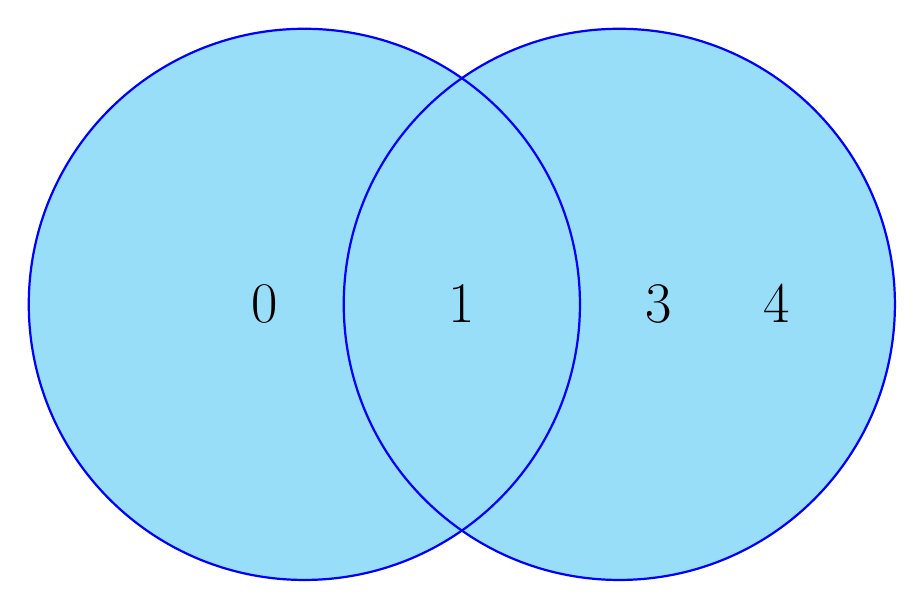
\begin{tikzpicture}
    \fill[cyan!40] (-2,0) circle (3.5cm);
    \fill[cyan!40] (2,0) circle (3.5cm);
    
    \draw[thick, draw=blue ] (-2,0) circle (3.5cm); 
    \draw[thick,draw=blue] (2,0) circle (3.5cm);  
    
    \node at (-2.5,0) {\huge $0$};
    \node at (0,0) {\huge $1$};
    \node at (2.5,0) {\huge $3$};
    \node at (4,0) {\huge $4$};
    
    
    
    
\end{tikzpicture}


\end{center}
L'unione raccoglie tutti gli elementi presenti in almeno uno dei due insiemi. L'elemento \(1\), che appartiene sia ad \(A\) che a \(B\), compare solo una volta nell'unione.
\end{esempio}

\propi{proprietà dell'unione}{
\item \(A \subseteq A\cup B\) e \(B \subseteq A\cup B\).
\item $A \cup B$ è il minimo dei soprainsiemi comuni di $A$ e $B$, cioè per ogni insieme $X$:
\[ X \supseteq A \ \text{ e } X \supseteq B \text{ implica } A \cup B \subseteq X \]
In altre parole, \(A \cup B\) è il più piccolo insieme che contiene sia \(A\) che \(B\).
\item La cardinalità dell'unione soddisfa la seguente relazione:
\[
    |A \cup B| = |A|+|B|- |A\cap B|
\]
}
\subsection{Intersezione}
\defn{Intersezione}{
Siano $A$ e $B$ due insiemi. L'intersezione di $A$ e $B$ si indica con $A \cap B$ ed è definita come segue:
\[
    A \cap B = \{ x\mid \left(x \in A\right) \land \left(x \in B\right)\}
\]
Cioè se $x \in A \cap B$ allora $x \in A$ e $x \in B$.

Due insiemi $A$ e $B$ si dicono \textbf{disgiunti} se $A\cap B = \emptyset$
}

L'intersezione raccoglie solo gli elementi comuni ai due insiemi. Se non hanno elementi in comune, la loro intersezione è l'insieme vuoto.
\begin{esempio}
    
 Sia $A = \{0,1\}$ e $B=\{1,3,4\}$, allora $ A \cap B= \{1\}$.
\[
    A \cap B
\]

 \begin{center}


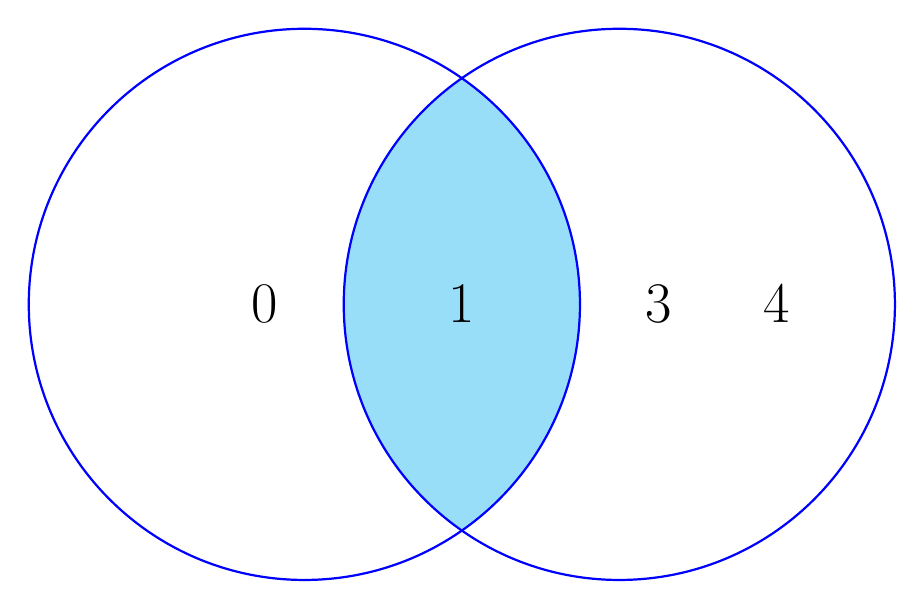
\begin{tikzpicture}
    
    \begin{scope}
        \clip (-2,0) circle (3.5cm);
        \fill[cyan!40] (2,0) circle (3.5cm);
    \end{scope}
    
    \draw[thick,  draw=blue] (-2,0) circle (3.5cm); 
    \draw[thick,  draw=blue] (2,0) circle (3.5cm);  
    
    \node at (-2.5,0) {\huge $0$};
    \node at (0,0) {\huge $1$};
    \node at (2.5,0) {\huge $3$};
    \node at (4,0) {\huge $4$};
    
\end{tikzpicture}
\end{center}
L'intersezione contiene solo gli elementi comuni ai due insiemi. Qui l'unico elemento che appartiene sia ad \(A\) che a \(B\) è \(1\).
\end{esempio}

\propi{Proprietà dell'intersezione}{
  \item L'intersezione di due insiemi è sempre contenuta in ciascuno dei due:
  \[
  A \cap B \subseteq A \quad \text{e} \quad A \cap B \subseteq B.
  \]

  \item Si può vedere \(A \cap B\) come il \textbf{massimo sottoinsieme comune} di \(A\) e \(B\): per ogni insieme \(X\):
  \[
  X \subseteq A \ \text{e} \ X \subseteq B \ \Longrightarrow \ X \subseteq A \cap B.
  \]
    In altre parole, \(A \cap B \) è il più grande insieme che è contenuto sia in \(A\) che in \(B\)
  \item La cardinalità dell'intersezione soddisfa la seguente catena di disuguaglianze:
  \[
  0 \;\le\; |A \cap B| \;\le\; \min\{|A|,\,|B|\} \;\le\; |A \cup B| \;\le\; |A|+|B|.
  \]

}


\subsection{Unione e intersezione di una famiglia di insiemi}

Siano $A_0, A_1, A_2, \ldots$ insiemi che sono sottoinsiemi di un insieme universale $U$, e dato un numero intero non negativo $n$, possiamo definire le seguenti operazioni di unione e intersezione di una collezione indicizzata di insiemi.

\begin{itemize}
    \item L'\textbf{unione finita} di una collezione di insiemi $A_0, A_1, A_2, \ldots, A_n$ è l'insieme degli elementi di $U$ che appartengono ad almeno uno degli insiemi $A_i$:
    \[
    \bigcup_{i=0}^{n} A_i = \{x \in U \ \mid \ \exists i \in \{0,1,\ldots,n\}, \ x \in A_i \}.
    \]
    
    \item L'\textbf{unione infinita} di una collezione di insiemi $A_0, A_1, A_2, \dots$ è l'insieme degli elementi di $U$ che appartengono ad almeno uno degli insiemi $A_i$:
    \[
    \bigcup_{i=0}^{\infty} A_i = \{x \in U \ \mid \exists i \in \mathbb{N}, \ x \in A_i \}
    \]

    \item L'\textbf{intersezione finita} di una collezione di insiemi $A_0, A_1, A_2, \dots, A_n$ è l'insieme degli elementi di $U$ che appartengono a tutti gli insiemi $A_i$ :
    \[
    \bigcap_{i=0}^{n} A_i = \{x \in U \ \mid \ \forall i \in \{0,1,\ldots,n\}, \ x \in A_i \}.
    \]
    
    \item L'\textbf{intersezione infinita} di una collezione di insiemi $A_0, A_1, A_2, \dots$ è l'insieme degli elementi di $U$ che appartengono a tutti gli insiemi $A_i$ :
    \[
    \bigcap_{i=0}^{\infty} A_i = \{x \in U \ \mid \forall i \in \mathbb{N}, \ x \in A_i \}.
    \]
\end{itemize}

\noindent Le operazioni di unione e intersezione indicizzate permettono di generalizzare la nozione di unione e intersezione a collezioni di insiemi che possono essere finite o infinite. Nel caso \textbf{dell'unione}, un elemento appartiene all'insieme risultante quando esiste almeno un sottoinsieme della collezione che contiene l'elemento. Nel caso \textbf{ dell'intersezione}, un elemento appartiene all'insieme risultante quando appartiene a tutti i sottoinsiemi della collezione.


\subsection{Complementazione }
\defn{Complementazione}{Sia $A \subseteq B$. La \textbf{complementazione} $B \setminus A$ di un sottoinsieme $A$ di $B$ è definita come:
\[
B\setminus A = \{x\mid x\in B \text{ e } x \not \in A\}
\]
si noti che : 
\[
\left(B\setminus A\right) \cap A = \emptyset \text{ e } \left(B\setminus A\right) \cup A = B
\]
}
\(B \setminus A \) è \virgolette{ciò che resta } di \(B\) dopo aver tolto tutti gli elementi che si trovano in \(A\); per questo è disgiunto da \(A\) e, insieme a \(A\), ricostruisce tutto \(B\).
\begin{esempio}
Se $A = \{3,4\}$ e $B=\{0,1,3,4\}$ allora:
\[
   B\setminus A = \{0,1\}
\]
Abbiamo rimosso da \(B\) solo gli elementi che appartengono ad \(A\), mantenendo gli altri.
\end{esempio} 



\subsection{Insieme complementare}
\defn{Insieme complementare}{Sia $U$ l'universo o dominio. L'insieme complementare di $A$, indicato con $\overline{A}$ è l'insieme di tutti gli elementi dell'universo $U$ che non appartengono ad $A$:
\[
\overline{A} = \{x \mid x\in U \text{ e } x \not \in A\}
\]
}
Il complementare \(A\) contiene \virgolette{tutto ciò che sta in \(U\) ma non in \(A\)}. Dipende sempre dall'insieme universo scelto: cambiare \(U\) cambia anche \(\overline{A}\).
\begin{center}
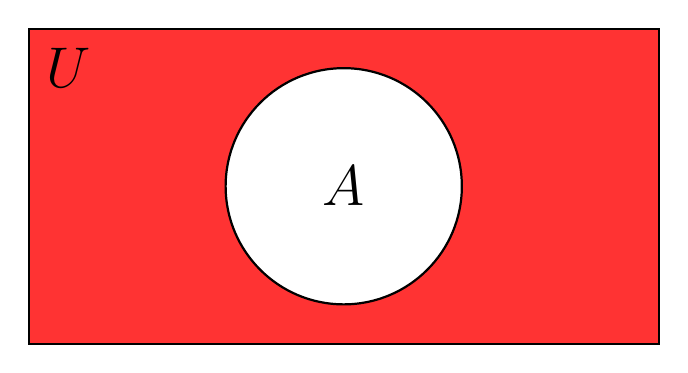
\begin{tikzpicture}
    \fill[red!80] (-4,-2) rectangle (4,2); 

    \fill[white] (0 ,0) circle (1.5cm); 
    \draw[thick] (0,0) circle (1.5cm); 


    \node at (0,0) {\huge $A$};
    \node at(-3.5,1.5) {\huge$U$};

    \draw[thick] (-4,-2) rectangle (4,2);
\end{tikzpicture}
\end{center}


% \begin{esempio}
    
% il complementare dell'insieme dei numeri primi
% rispetto ai numeri naturali è l'insieme che comprende i numeri
% $0, 1$ e tutti i numeri maggiori o uguali a $2$ che sono composti.
% \end{esempio}  

\subsection{Differenza}
\defn{Differenza}{Dati due insiemi $A$ e $B$ definiamo la \textbf{differenza}

\[
A\setminus B = \{x \in A \land x \not \in B\}
\]
 Si noti che, in generale, la differenza non è un'operazione simmetrica. Infatti, in generale vale
\[
A \setminus B \neq B \setminus A,
\]
tranne nel caso particolare in cui $A = B$.
Inoltre, la differenza è collegata all'intersezione dalla seguente proprietà fondamentale:
\[
(A \setminus B) \cup (A \cap B) = A.
\]

}
\(A \setminus B\) contiene gli elementi che si trovano in \(A\) ma non in \(B\). Insieme alla parte comune \( A \cap B\) ricostruisce tutto \(A\).




\begin{center}
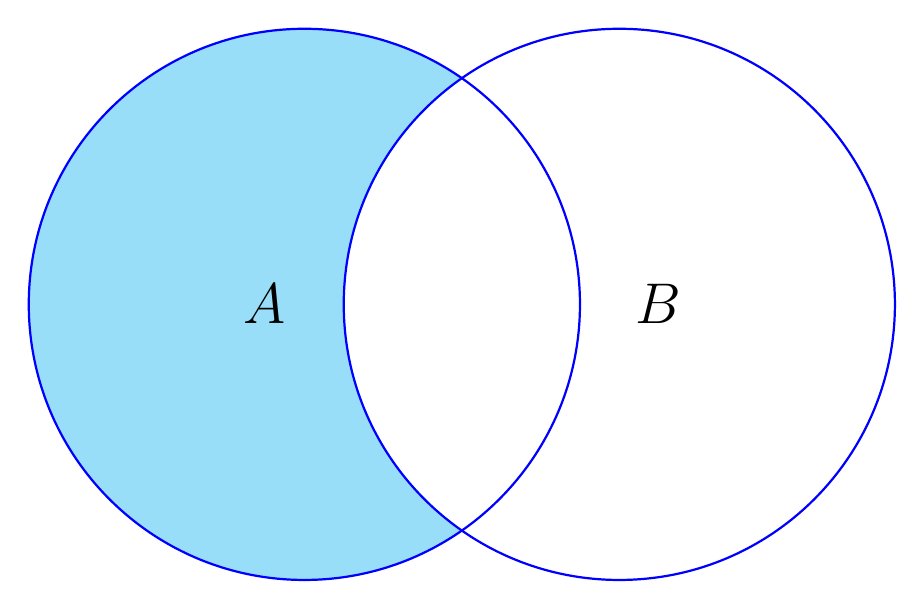
\begin{tikzpicture}
    % Differenza A \ B
    \begin{scope}
        % Primo clip: prendi A
        \clip (-2,0) circle (3.5cm);
        % Secondo clip: escludi B
        \fill[cyan!40] (-6,-4) rectangle (6,4);
        \clip (2,0) circle (3.5cm);
        \fill[white] (-6,-4) rectangle (6,4);
    \end{scope}

    % Contorni dei cerchi
    \draw[thick, blue] (-2,0) circle (3.5cm); 
    \draw[thick, blue] ( 2,0) circle (3.5cm);  

    % Etichette
    \node at (-2.5,0) {\huge $A$};
    \node at ( 2.5,0) {\huge $B$};
\end{tikzpicture}
\end{center}

\subsection{Differenza simmetrica}
\defn{Differenza simmetrica}{
Dati due insiemi $A$ e $B$ definiamo la \textbf{differenza simmetrica}
\[
    A \ \Delta \ B = \left(A \setminus B\right) \cup (B \setminus A)
\]
}
La differenza simmetrica contiene tutti gli elementi che appartengono ad \(A\) o a \(B\), ma non a entrambi. Esclude quindi la parte in comune.
\begin{center}
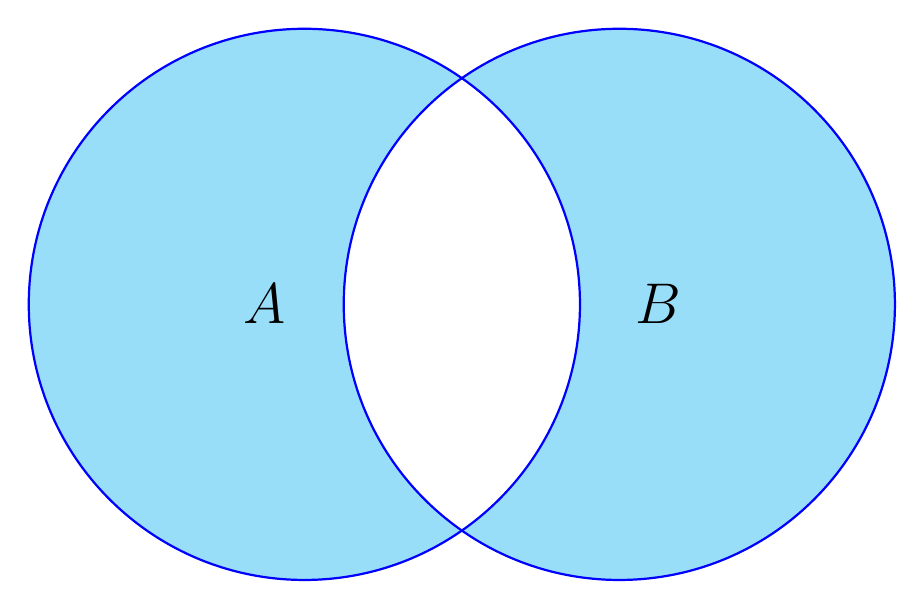
\begin{tikzpicture}
    % Parte A \ B
    \begin{scope}
        \clip (-2,0) circle (3.5cm);
        \fill[cyan!40] (-6,-4) rectangle (6,4);
        \clip (2,0) circle (3.5cm);
        \fill[white] (-6,-4) rectangle (6,4);
    \end{scope}

    % Parte B \ A
    \begin{scope}
        \clip (2,0) circle (3.5cm);
        \fill[cyan!40] (-6,-4) rectangle (6,4);
        \clip (-2,0) circle (3.5cm);
        \fill[white] (-6,-4) rectangle (6,4);
    \end{scope}

    % Contorni
    \draw[thick, blue] (-2,0) circle (3.5cm); 
    \draw[thick, blue] ( 2,0) circle (3.5cm);  

    % Etichette
    \node at (-2.5,0) {\huge $A$};
    \node at ( 2.5,0) {\huge $B$};
\end{tikzpicture}
\end{center}



\subsection{Proprietà delle operazioni sugli insiemi}
Le operazioni sugli insiemi soddisfano le seguenti proprietà: per
ogni sottoinsieme $A$, $B$ e $C$ di un insieme $ X$.

\propi{Idempotenza}{
\item$ A \cap A = A $ e $A \cup A = A$
\item$ A \cup \emptyset = A $ e $A \cap \emptyset = \emptyset$
\item$ A \cup X= X$ e $A \cap X = A$
}

\begin{osservazione}
    Unire o intersecare un insieme con se stesso o con l'insieme vuoto non cambia sostanzialmente il contenuto.
\end{osservazione}
\propi{Assorbimento}{\item $A \cup \left(A \cap B\right)= A$ \quad \text{e} \quad $A \cap \left(A \cup B\right)=A$ }
\begin{osservazione}
L'insieme \virgolette{più grande} assorbe quello più piccolo : aggiungere a \(A\) che è già contenuto in \(A\) non lo cambia.
\end{osservazione}






\propi{Proprietà commutativa}{
    \item $A \cup B = B \cup A$ e $A \cap B = B \cap A$
}

\propi{Proprietà associativa}{
    \item $(A \cup B) \cup C = A \cup (B \cup C) = A \cup B \cup C$
    \item $(A \cap B) \cap C = A \cap (B \cap C) = A \cap B \cap C$
}

\propi{Proprietà distributiva}{
    \item $A \cap (B \cup C) = (A \cap B) \cup (A \cap C)$
    \item $A \cup (B \cap C) = (A \cup B) \cap (A \cup C)$
}

\begin{osservazione}
    Le proprietà commutativa,associativa e distributiva mostrano che unione e intersezione si comportano in modo simile a somma e prodotto nell'aritmetica.
\end{osservazione}
Sia $U$ l'insieme universo:
\propi{Complementazione }{
    \item $A \cup \overline{A} = U$ e $A \cap \overline{A} = \emptyset$
}
Le leggi di De Morgan che abbiamo già visto applicate all'algebra
booleana, mettono in relazione le operazioni di unione e
intersezione con il complementare:
\propi{Leggi di De Morgan}{
    \item $\overline{A \cup B} = \overline{A} \cap \overline{B}$
    \item $\overline{A \cap B} = \overline{A} \cup \overline{B}$
}


\section{Partizione}


\defn{Disgiunzione}{
    Due insiemi si dicono disgiunti se e solo se non hanno alcun elemento in comune.
\[
A \cap B = \emptyset
\]
}
 La loro intersezione è vuota: non esiste nessun elemento che appartenga contemporaneamente ad entrambi.

\begin{esempio}
Sia $A = \{1, 3, 5\}$ e $B = \{2, 4, 6\}$. Gli insiemi $A$ e $B$ sono disgiunti?
\[
A \cap B = \{1, 3, 5\} \cap \{2, 4, 6\} = \emptyset
\]
\end{esempio} 
Tutti gli elementi di \(A\) sono dispari e tutti quelli di \(B\) sono pari, quindi non possono coincidere: per questo l'intersezione è vuota e \(A\) e \(B\) sono disgiunti.

% \subsection*{Insiemi mutuamente disgiunti}
\defn{Insiemi mutuamente disgiunti}{
Gli insiemi $A_1, A_2, \dots, A_m$ sono mutuamente disgiunti se e solo se, presi due insiemi qualunque $A_i$ e $A_j$, con $i \neq j$, non hanno elementi in comune.
Formalmente:
\[
A_i \cap A_j = \emptyset \quad \text{per ogni} \ i \neq j
\]
Non solo ogni coppia è disgiunta, ma questo vale per tutte le coppie possibili della famiglia: nessun elemento compare in più di un  insieme. 
}

\begin{esempio}
    Sia 
    \[
    A_1 = \{ 0,1\} , \quad A_2= \{2,3\}  A_3 = \{4,5\}
    \]
    Allora $A_1, A_2, A_3 $ sono mutuamente disgiunti perché
    \[
        A_1 \cap A_2 = A_1 \cap A_3 = A_2 \cap A_3  = \emptyset
    \]
    Ogni coppia di insiemi ha intersezione vuota: nessun elemento compare in più di un insieme. Si noti che non è sufficiente verificare una sola coppia, ma tutte le possibili coppie distinte.
\end{esempio}




\defn{Partizione}{
Una \textbf{partizione} di un insieme $X$ è una famiglia di sottoinsiemi non vuoti 
$A_1, A_2, \ldots, A_k$ tali che:  
\begin{itemize}
    \item gli insiemi $A_i$ sono a due a due disgiunti, cioè 
    \[
    A_i \cap A_j = \emptyset \quad \text{per ogni } i \neq j \,,
    \]
    \item l'unione dei sottoinsiemi ricopre l'intero insieme $X$, cioè 
    \[
    A_1 \cup A_2 \cup \cdots \cup A_k = X.
    \]
    
\end{itemize}
In altre parole, una partizione suddivide l'insieme $X$ in sottoinsiemi non sovrapposti che, presi tutti insieme, contengono esattamente gli elementi di $X$: ogni elemento di $X$ appartiene a uno e un solo blocco della partizione.

}

\begin{esempio}
    Sia $X = \{1,2,3,4,5,6\}$. Verificare se $\{A_1, A_2, A_3\}$ con 
$A_1 = \{1,2\}$, $A_2 = \{3,4\}$, $A_3 = \{5,6\}$ è una partizione di $X$.
\medskip

\begin{strategiabox}
    Dobbiamo verificare le due condizioni della definizione: disgiunzione a coppie e copertura di \(X\).
\end{strategiabox}

\begin{itemize}
    \item $A_1 \cap A_2 = A_1 \cap A_3 = A_2 \cap A_3 = \emptyset$ \quad (disgiunti a coppie)
    \item $A_1 \cup A_2 \cup A_3 = \{1,2,3,4,5,6\} = X$ \quad (copertura)
\end{itemize}
Entrambe le condizioni sono soddisfatte, quindi $\{A_1, A_2, A_3\}$ formano una partizione di $X$.
\end{esempio}

\section{Dimostrazioni}
Per dimostrare che due insiemi $A$ e $B$ hanno gli stessi elementi, 
cioè che $A = B$, è necessario verificare entrambe le seguenti condizioni:
\begin{itemize}
    \item $A$ è un sottoinsieme di $B$, cioè $A \subseteq B$;
    \item $B$ è un sottoinsieme di $A$, cioè $B \subseteq A$.
\end{itemize}

\exm{Sia $X$ un insieme. Dimostrare che, per tutti i sottoinsiemi $A$ e $B$ di $X$, 
vale la seguente proprietà di assorbimento:
\[
A \cup (A \cap B) = A
\]
}{

% Dobbiamo dimostrare che $A \cup (A \cap B) \subseteq A$ e $A \subseteq A \cup (A \cap B)$.

\begin{strategiabox}
Dimostriamo l'uguaglianza per \textbf{doppia inclusione}:
\[
A \cup (A \cap B) \subseteq A \quad \text{e} \quad  A \subseteq A \cup (A \cap B)
\]
\end{strategiabox}

\begin{itemize}
    \item (\(\subseteq\)) Dimostriamo che $A \cup (A \cap B) \subseteq A$.  
    Infatti, se $x \in A \cup (A \cap B)$, allora $x \in A$ oppure $x \in A \cap B$ (per definizione di $\cup$).  
    Nel primo caso, $x \in A$ e abbiamo finito.  
    Nel secondo caso, da $x \in A \cap B$ segue che $x \in A$ e $x \in B$ (per definizione di $\cap$).  
    In entrambi i casi, dunque, $x \in A$.

    \item (\(\supseteq\)) Dimostriamo che $A \subseteq A \cup (A \cap B)$.  
    Se $x \in A$, allora $x$ appartiene a ogni sovrainsieme di $A$, in particolare ad $A \cup (A \cap B)$.
\end{itemize}
Avendo mostrato entrambe le inclusioni, si ottiene:  \[A\cup (A \cap B) = A\]
}

\medskip

\exm{Sia $X$ un insieme. Dimostrare che, per tutti i sottoinsiemi $A$, $B$ e $C$ di $X$, 
vale la seguente proprietà distributiva:
\[
A \cup (B \cap C) = (A \cup B) \cap (A \cup C)
\]
}{
\begin{strategiabox}
     Dimostriamo l'uguaglianza per doppia inclusione.
\end{strategiabox}

\begin{itemize}
    \item (\(\subseteq\)) Dimostriamo che $A \cup (B \cap C) \subseteq (A \cup B) \cap (A \cup C)$.  
    Infatti, se $x \in A \cup (B \cap C)$, allora $x \in A$ oppure $x \in B \cap C$.  
    Se $x \in A$, allora $x \in A \cup B$ e $x \in A \cup C$, quindi $x \in (A \cup B) \cap (A \cup C)$.  
    Se invece $x \notin A$, allora $x \in B \cap C$, cioè $x \in B$ e $x \in C$.  
    Da $x \in B$ segue $x \in A \cup B$, e da $x \in C$ segue $x \in A \cup C$.  
    Quindi in ogni caso $x \in (A \cup B) \cap (A \cup C)$.

    \item (\(\supseteq\)) Dimostriamo che $(A \cup B) \cap (A \cup C) \subseteq A \cup (B \cap C)$.  
    Se $x \in (A \cup B) \cap (A \cup C)$, allora $x \in A \cup B$ e $x \in A \cup C$.  
    Se $x \in A$, allora chiaramente $x \in A \cup (B \cap C)$.  
    Se invece $x \notin A$, da $x \in A \cup B$ segue $x \in B$, e da $x \in A \cup C$ segue $x \in C$.  
    Quindi $x \in B \cap C$, e dunque $x \in A \cup (B \cap C)$.
\end{itemize}

Poiché abbiamo dimostrato entrambe le inclusioni, segue che :
\[A \cup (B \cap C) = (A \cup B) \cap (A \cup C)\].
}



\newpage

\section{Esercizi}




\begin{esercizio}
Dare una definizione matematica, tramite una proprietà, dei seguenti insiemi: 
\begin{enumerate}
    \item L'insieme di tutti i numeri pari 
    \item L'insieme di tutti i numeri dispari 
    \item L'insieme di tutti i numeri naturali che sono multipli di 5
    \item L'insieme di tutti i numeri naturali il cui quadrato è minore di 21
\end{enumerate}  
Sia l'insieme dei numeri naturali $\mathbb{N}$ il dominio di riferimento.
\end{esercizio}

\begin{soluzione}
\begin{enumerate}
    \item  $X = \{ 2x \mid x \in \mathbb{N}  \}$  
    oppure $X = \{ x \in \mathbb{N} \mid x = 2n \wedge n \in \mathbb{N}  \}$
    \item $X = \{ 2x+1 \mid x \in \mathbb{N}  \}$
    \item $X = \{ x  \mid x \in \mathbb{N} \wedge x = 5n \wedge n \in \mathbb{N} \}$ 
    \item $X = \{ x  \mid x \in \mathbb{N} \wedge x^2 < 21 \}$
\end{enumerate}
\end{soluzione}

% ---------

\begin{esercizio}
Per ognuna delle seguenti coppie di insiemi, $A$ e $B$, dire quando l'enunciato \virgolette{$A \subseteq B$} è vero o falso:
\begin{enumerate}
    \item $A = \{ 2,4,8 \}$, $B = \{ m \in \mathbb{N} \mid m \ \grave{e} \ un \ numero \ pari \}$
    \item $A = \{3,7,1025 \}$,  $B = \{ m \in \mathbb{N} \mid m = 2^n -1 \ per \ qualche \ numero \ n \in \mathbb{N}\}$
    \item $A = \{ 0 \}$, $B = \emptyset$
    \item $A = \emptyset$, $B = \{ 0 \}$
\end{enumerate}    
\end{esercizio}

\begin{soluzione}
\begin{enumerate}
    \item Vero
    \item Falso
    Sia $1025 = 2^n - 1 $. Perché l'uguaglianza valga poniamo $2^n = 1026$.\ 
    Quanto vale $n$? $n = log_2 (1026) = 10.002815015607053 \not\in \mathbb{N}$ 
    \item Falso
    \item Vero 
    L'insieme vuoto è un sottoinsieme (improprio) di qualsiasi insieme.\\
\end{enumerate}
\end{soluzione}

% ----------------

\begin{esercizio}
Provare che le seguenti affermazioni sono false esibendo dei controesempi espliciti:
\begin{itemize}
    \item $A\cap B = A \cap C\Rightarrow B = C$
    \item $(B\cup A)\cap C = B\cup (A\cap C)$
\end{itemize}
\end{esercizio}

\begin{soluzione}
\begin{itemize}
    \item $A\cap B = A \cap C\Rightarrow B = C$\\
    Prendiamo per esempio $A=\emptyset$, $B=\{1\}$, $C=\{2\}$ dunque $A\cap B = A\cap C$ ma questo non implica $B=C$ che sono evidentemente diversi
    \item $(B\cup A)\cap C = B\cup (A\cap C)$\\
    Prendiamo per esempio $A=B=\{1\}$, $C=\emptyset$ dunque 
    $$(B\cup A)\cap C = \emptyset \neq B\cup (A\cap C) = \{1\}$$
\end{itemize}
\end{soluzione}

% ----------

\begin{esercizio}
Dato l'insieme $X = \{ a, b, c \}$, definire l'insieme delle parti di $X$.
\end{esercizio}

\begin{soluzione}
\[
\mathcal{P}(X) = \{ \emptyset, \{ a \}, \{ b \}, \{ c \}, \{ a,b \}, \{ a,c \}, \{ b,c \}, \{ a, b, c \} \}
\]
\end{soluzione}

% ---------------

\begin{esercizio}
Siano $X=\mathbb{R}$, $A=\{x\in\mathbb{R} ~|~ x^2+x-2=0\}$, $B=\{1, -2\}$ e $C=\{1, \{2,3\}\}$.
\begin{itemize}
    \item Determinare  l'insieme delle parti di $B$ e l'insieme delle parti di $C$
    \item Dire quali delle seguenti affermazioni sono vere e quali false:\\
\end{itemize}

\begin{center}
    \begin{tabular}{lclclcl}
        \medskip
        $\{1\}\not\subseteq A $ &~& $1\in C$       &~& $\{1\}\in A$   &~& $2\in C$\\
        \medskip
        $1\subseteq A$          &~& $3\in C$       &~& $1\in A$       &~& $\{1\}\in C$\\
        \medskip
        $A\subseteq B$          &~& $\{2,3\}\in C$ &~& $B\subseteq A$ &~& $\{2\}\in C$\\
    \end{tabular}
\end{center}
\end{esercizio}

\begin{soluzione}
\begin{itemize}
    \item $\mathcal{P}(B)=\{\emptyset, \{1\}, \{-2\}, B\}$\\
    $\mathcal{P}(C)=\{\emptyset, \{1\}, \{\{2,3\}\}, C \}$
    \item Sono corrette soltanto le seguenti cinque affermazioni: $1\in C,\ 1\in A,\ \{2, 3\}\in C,\ A\subseteq B,\ B\subseteq A $ le altre sono false perchè:
    \begin{itemize}
        \item $\{1\}\not\subseteq A $ essendo $1$ un elemento di $A$, l'insieme $\{1\}$ è effettivamente contenuto uguale in $A$
        \item $\{1\}\in A$ l'insieme $\{1\}$ NON fa parte degli elementi di $A$
        \item $2\in C$ l'elemento $2$ NON fa parte degli elementi di $C$
        \item $1\subseteq A$ essendo l'inclusione una relazione binaria definita tra insiemi l'elemento $1$ NON è sottoinsieme di $A$
        \item $3\in C$, $3$ NON fa parte degli elementi di $C$
        \item $\{1\}\in C$, l'insieme $\{1\}$ NON fa parte degli elementi di $C$
        \item $\{2\}\in C$, l'insieme $\{2\}$ NON fa parte degli elementi di $C$
    \end{itemize}
\end{itemize}
\end{soluzione}

% -------------

\begin{esercizio}
Sia $X = \{ 1,2,3 \}$. Scrivere tutte le possibili partizioni di $X$. 
\end{esercizio}

\begin{soluzione}
Esistono 5 possibili partizioni di $X$: 
\begin{enumerate}
    \item $\{1 \}, \{ 2 \}, \{ 3 \}$
    \item $\{1,2 \}, \{3 \}$
    \item $\{1,3 \}, \{ 2 \}$
    \item $\{ 2,3 \}, \{ 1 \}$
    \item $\{ 1,2,3 \}$
\end{enumerate}
\end{soluzione}

% ----------

\begin{esercizio}
Per ogni $n\in\mathbb{N}$, siano $A_n=\{x\in \mathbb{N} | x\neq n+1\}$, $B_n=\{x\in\mathbb{N} | x\neq 2n\}$, $C_n=\{x\in\mathbb{N} | x\neq 2n+3\}$.
Calcolare:
\begin{center}
    \begin{tabular}{lcl}
        \medskip
        $\bigcup_{n\in\mathbb{N}}A_n$ && $\bigcap_{n\in\mathbb{N}}A_n$\\
        \medskip
        $\bigcup_{n\in\mathbb{N}}B_n$ && $\bigcap_{n\in\mathbb{N}}B_n$\\ 
        \medskip
        $\bigcup_{n\in\mathbb{N}}C_n$ && $\bigcap_{n\in\mathbb{N}}C_n$\\
    \end{tabular}
\end{center}

\end{esercizio}

\begin{soluzione}
    \begin{itemize}
\item $\bigcup_{n\in\mathbb{N}}A_n = \mathbb{N}$ 
\item $\bigcap_{n\in\mathbb{N}}A_n = \{0\}$
\item $\bigcup_{n\in\mathbb{N}}B_n = \mathbb{N}$
\item $\bigcap_{n\in\mathbb{N}}B_n = \{x\in\mathbb{N}\ |\ x\ \text{è\ dispari}\}$
\item $\bigcup_{n\in\mathbb{N}}C_n \mathbb{N}$
\item $\bigcap_{n\in\mathbb{N}}C_n = \{x\in\mathbb{N}\ |\ x\ \text{è\ pari} \vee x=1\}$
\end{itemize}

\end{soluzione}

% ---------

\begin{esercizio}
Siano $D$ e $P$ i sottoinsiemi dei numeri dispari e pari, rispettivamente. Dimostrare che $\{D, P\}$ è una partizione di $\mathbb{N}$.
\end{esercizio}

\begin{soluzione}
Si dice partizione di $X$ una famiglia di suoi sottoinsiemi tali che: nessuno di essi è vuoto, sono due a due disgiunti e la loro unione è tutto $X$.
Per verificare quanto sopra dobbiamo verificare le seguenti condizioni (date dalla definizione):
\begin{enumerate}
    \item $D\neq \emptyset$
    \item $P\neq \emptyset$
    \item $P\cap D = \emptyset$
    \item $P\cup D= \mathbb{N}$
\end{enumerate}
Esistono in $\mathbb{N}$ sia numeri pari che dispari di conseguenza le condizioni 1. e 2. sono vere, non esistono numeri che siano allo stesso tempo sia pari che dispari di conseguenza anche 3. è verificata, ed unendo i numeri pari appartanenti a $\mathbb{N}$ ed i numeri dispari appartenenti a $\mathbb{N}$ otteniamo l'intero insieme dei numeri naturali. \\
\end{soluzione}

% -------------

\begin{esercizio}
Determinare se il seguente enunciato è vero o falso e giustificare la risposta.
Utilizzare le proprietà delle relazioni e delle variabili coinvolte. 
\begin{center} 	 
    Se $A \subseteq B$ e $C \subseteq D$ allora $A \times C \subseteq B \times D$. 
\end{center}
\end{esercizio}

\begin{soluzione}
Notare che l'enunciato può essere riscritto come: $A \subseteq B \wedge C \subseteq D \Rightarrow A \times C \subseteq B \times D$.
L'enunciato è vero.  Se $(a,c) \in A \times C$ allora $a \in A$. Dato che $A \subseteq B$ allora abbiamo che $a \in B$. In modo simile, $c \in C$ e $C \subseteq D$ implica che $c \in D$. Quindi se $a \in B$ e $c \in D$ allora $(a,c) \in B \times D$ e possiamo concludere che $A \times C \subseteq B \times D$. \\
\end{soluzione}
% ----------

\begin{esercizio}
Costruire un contro-esempio per il seguente enunciato. 
\begin{center}
    $A \cap (B \cup C) = (A \cap B) \cup C$ \hspace*{0,5cm} $\forall A, B, C$
\end{center}
\end{esercizio}

\begin{soluzione}
Se $A = \{ 1,2 \}, B = \{ 1 \}$ e $C = \{ 3 \}$ allora: 
\begin{itemize}
    \item $A \cap (B \cup C) = \{ 1,2 \} \cap \{ 1,3 \} = \{ 1 \}$
    \item $(A \cap B) \cup C = (\{ 1, 2 \} \cap \{ 1 \}) \cup \{ 3 \} = \{ 1, 3 \}$
\end{itemize}
Quindi i due insiemi sono diversi (l'enunciato non è vero per ogni insieme $A,B$ e $C$). 
\end{soluzione}

% -------------

\begin{esercizio}
Determinare se il seguente enunciato è vero o falso e giustificare la risposta.
Utilizzare le proprietà delle relazioni e delle variabili coinvolte. 
\begin{center}
    $(A \cap B) \cup C = A \cap (B \cup C) \Leftrightarrow C \subseteq A$
\end{center} 
\end{esercizio}

\begin{soluzione}
\begin{itemize}
    \item[$\Leftarrow$]  Assumiamo che $C\subseteq A$ sia vera. Per la proprietà distributiva $(A \cap B) \cup C = (A \cup C) \cap (B \cup C)$. Siccome $C \subseteq A$, abbiamo che $A \cup C = A$ e quindi $(A \cup C) \cap (B \cup C) = A \cap (B \cup C)$. Ciò significa che abbiamo $(A \cap B) \cup C = A \cap (B \cup C)$. 
    \item[$\Rightarrow$] Assumiamo che  $(A \cap B) \cup C = A \cap (B \cup C)$ sia vera. Per le proprietà di unione e intersezione abbiamo che: $C \subseteq (A \cap B) \cup C$ e $A \cap (B \cup C) \subseteq A$. Per le assunzioni fatte in precedenza e per la transitività delle relazioni tra sottoinsiemi, otteniamo $C \subseteq A$.  
\end{itemize} 

\end{soluzione}

% -----------

\begin{esercizio}
Dimostrare oppure confutare mediante controesempi le seguenti uguaglianze tra insiemi:
\begin{enumerate}
    \item $\mathcal{P}(A) \cap \mathcal{P}(B)=\mathcal{P}(A\cap B)$
    \item $\mathcal{P}(A)\cup\mathcal{P}(B)=\mathcal{P}(A\cup B)$
\end{enumerate}
\end{esercizio}

\begin{soluzione}
La relazione in 1. è vera e lo dimostriamo come segue:
\begin{itemize}
\item[$\Rightarrow$] $\mathcal{P}(A) \cap \mathcal{P}(B) \rightarrow \mathcal{P}(A\cap B)$\\
Per definizione di insieme delle parti sappiamo che per un qualunque insieme $X$ vale quanto segue $$X\in\mathcal{P}(A) \Leftrightarrow X\subseteq A$$
Assumiamo che la prima parte dell'implicazione sia vera dunque avremo che $X\in(\mathcal{P}(A)\cap\mathcal{P}(B))$ che corrisponde a scrivere $X\in\mathcal{P}(A)\wedge X\in\mathcal{P}(B)$ che equivale a scrivere $X\subseteq A\wedge X\subseteq B$, dunque essendo che $X$ è contenuto sia in $A$ che in $B$ sarà contenuto anche della loro intersezione, quindi $X\subseteq (A\cap B)$ che implica $$X\in\mathcal{P}(A\cap B)$$ che è esattamente ciò che volevamo ottenere.

\item[$\Leftarrow$] $\mathcal{P}(A\cap B) \rightarrow \mathcal{P}(A) \cap \mathcal{P}(B)$\\
Seguiamo un ragionamento analogo ed assumiamo che la prima parte dell'implicazione sia vera dunque avremo che per un qualunque insieme $X$ vale quanto segue $X\in\mathcal{P}(A\cap B)$ che equivale a scrivere $X\subseteq (A\cap B)$ ma per essere sottoinsieme dell'intersezione di $A$ e $B$ dovrà essere sottoinsieme sia di $A$ che di $B$, ossia $X\subseteq A\wedge X\subseteq B$ che per definizione di insieme delle parti sappiamo significare $X\in\mathcal{P}(A)\wedge X\in\mathcal{P}(B)$ dunque avremo che $X\in(\mathcal{P}(A)\cap \mathcal{P}(B))$ che è esattamente ciò che volevamo ottenere.
\end{itemize}
\qed
\bigskip

\noindent La relazione in 2. è falsa e ci basta trovare un controesempio per dimostrarlo. Per esempio, prendiamo $A=\{1\}$ e $B=\{2\}$, notiamo infatti che 
$$\mathcal{P}(A)\cup\mathcal{P}(B) = \{\emptyset, A, B\} \neq \mathcal{P}(A\cup B) = \{\emptyset, A, B, \{1,2\} \}$$
Volendo dimostrarlo per assurdo possiamo procedere come segue. Premesso che dire che $\mathcal{P}(A)\cup \mathcal{P}(B)=\mathcal{P}(A\cup B)$ significa dire che: 
$$\mathcal{P}(A)\cup \mathcal{P}(B)\subseteq \mathcal{P}(A\cup B) \wedge \mathcal{P}(A\cup B)\subseteq  \mathcal{P}(A)\cup \mathcal{P}(B)$$
Assumiamo per assurdo che $\mathcal{P}(A\cup B)\subseteq  \mathcal{P}(A)\cup \mathcal{P}(B)$. 
Per definizione di insieme delle parti abbiano che $$(A\cup B) \in \mathcal{P}(A\cup B)$$ ma secondo la nostra ipotesi dovrebbe valere anche quanto segue: 
$$(A\cup B)\in\mathcal{P}(A) \vee (A\cup B)\in\mathcal{P}(B)$$
ossia
$$(A\cup B)\subseteq A \vee (A\cup B)\subseteq B$$
Questo risulta però vero se e solo se $A=B$, essendo che $A=B$ non fa parte delle assunzioni del nostro enunciato, abbiamo raggiunto una contraddizione per cui l'enunciato risulta essere, in generale, falso. \qed\\
\end{soluzione}

% --------------

\begin{esercizio}
Determinare se il seguente enunciato è vero o falso e giustificare la risposta. Utilizzare la tecnica di dimostrazione per contraddizione.
\begin{center} 
    \virgolette{Non esiste un numero razionale strettamente positivo, più piccolo di tutti gli altri}.
\end{center}
\end{esercizio}

\begin{soluzione}
L'enunciato è vero. Supponiamo che non lo sia.  Supponiamo quindi che esista un numero razionale positivo più piccolo di tutti gli altri. Sia questo numero $r > 0$. Prendiamo ora $\dfrac{r}{2}$, esso è ancora razionale, è ancora positivo ma è evidentemente più piccolo di $r$.  Ciò contraddice la supposizione fatta. L'enunciato di partenza è quindi vero per contraddizione. \\
\end{soluzione}

% -----------

\begin{esercizio}
Siano $A$ e $B$ due insiemi.  Determinare se la seguente uguaglianza è vera o falsa e giustificare la risposta. Utilizzare la tecnica di dimostrazione per contraddizione.
    $$(A - B) \cap (B - A) = \varnothing$$
\end{esercizio}

\begin{soluzione}
L'uguaglianza è vera.\\
Supponiamo che non la sia.
Supponiamo quindi che questa intersezione non sia vuota e che esista un elemento $x$ appartenente a questa intersezione.
Supponiamo inoltre che entrambi gli insiemi appartengano ad un insieme universo $U$.
Scriviamo ora $A-B$ come $A \cap \overline{B}$ dove $\overline{B}$ è il complementare di $B$ rispetto all'insieme universo $U$ a cui $A$ e $B$ appartengono.
Analogamente, poniamo $B-A=B \cap \overline{A}$. Ma, se $x$ appartiene all'intersezione di questi insiemi, significa che: $x$ appartiene ad $A$ ma anche ad $\overline{A}$.
Inoltre $x$ appartiene a $B$, ma anche a $\overline{B}$. Ciò contraddice la supposizione fatta. 
Infatti, si noti che $\overline{B} = U-B$, quindi $\overline{B}$ è l'insieme degli elementi di $U$ che non appartengono a $B$. 
Non può esistere quindi un $x$ appartenente sia a $B$ che a $\overline{B}$  (lo stesso vale per $A$).
L'uguaglianza di partenza è quindi vera per contraddizione. \\
\end{soluzione}

% -----------

\begin{esercizio}
Siano $A,B$ e $C$ tre insiemi. Determinare se la seguente relazione è vera o falsa e giustificare la risposta. Utilizzare le proprietà  delle relazioni e delle variabili coinvolte.

    $$(A-B) - C \subseteq A - C$$
\end{esercizio}

\begin{soluzione}
Supponiamo che $x$ appartenga ad $(A-B) - C$. Ne consegue che  $x \in A - B$ e che $x \not\in C$. Ma ciò significa affermare che $x \in A$, $x \not\in B$ e $x \not\in C$. Se $x \in A$ e $x \not\in B$ implica che $x \in A-C$. Quindi $(A-B) - C \subseteq A - C$. \\
\end{soluzione}

% --------------

\begin{esercizio}
Siano $A,B$ e $C$ tre insiemi. Determinare se la seguente uguaglianza è vera o falsa e giustificare la risposta. Utilizzare le proprietà delle operazioni fra insiemi.
    $$(A-C) \cap (C-B) = \varnothing$$
\end{esercizio}

\begin{soluzione}
\begin{align*}
    (A-C) \cap (C-B) & = (A \cap \overline{C}) \cap (C \cap \overline{B})  && \text{(definizione)}\\
    & = (\overline{C} \cap C) \cap (A \cap \overline{B})  && \text{(associatività)}\\
    & = \varnothing \cap (A \cap \overline{B})  && (S-S = \varnothing)\\
    & = \varnothing  \\
\end{align*}
\end{soluzione}

% ----------------

\begin{esercizio}
Siano $A,B$ e $C$ tre insiemi. Determinare se la seguente uguaglianza è vera o falsa e giustificare la risposta. Utilizzare le proprietà delle operazioni fra insiemi.

    $$(B-A) \cup (C-A) = (B \cup C) - A$$
\end{esercizio}

\begin{soluzione}
\begin{align*}
    (B-A) \cup (C-A) & = (B \cap \overline{A}) \cup (C \cap \overline{A}) &&\text{(definizione)}\\
    & = (B \cup C) \cap \overline{A} &&\text{(distributività)}\\
    & = (B \cup C)  - A &&\text{(definizione)}
\end{align*}
\end{soluzione}